\documentclass[a4paper,10pt]{article}
\usepackage[utf8]{inputenc}
\usepackage{setspace}
\usepackage{amsmath,calc,amssymb,graphicx}
\usepackage{tcolorbox}
\DeclareGraphicsExtensions{.pdf,.png,.jpg}
% Text layout
\topmargin -2.0cm
\oddsidemargin 0.5cm
\evensidemargin 0.5cm
\textwidth 15cm 
\textheight 24cm
\usepackage{cite}
%opening
\title{Exercises CPM\\ \large Course Seignosse 2018, day 4}
\author{Renske Vroomans}
\date{}

\begin{document}

\maketitle
%\section*{Introduction}
These exercises are meant to give you an intuition about the dynamics of the CPM. Feel free to explore any of the parameters of the model as much as you like, to see how they influence the behaviour.
The questions are just there to guide you to some interesting places. It has been heavily inspired by exercises from the EMBO course organised by dr. 
Stan Mar\'ee and dr. Ver\^onica Grieneisen at the John Innes Center in Norwich; they are also an excellent resource for anything CPM related.

\section*{Getting started}
\subsection*{Linux basics}
If Linux is new to you, using the terminal may be quite daunting. Here are some handy commands to get you started:
\begin{itemize}
 \item \texttt{cd} \textit{dirname} ~~ will move you into this directory (cd=``change directory'') Press tab after \texttt{cd} to see options and to autocomplete the dirname. \texttt{cd} .. will move you to a higher directory, and just \texttt{cd} will take you to the home dir.
 \item \texttt{ls}  ~~ lists the files in the current directory.
 \item \texttt{gedit} \textit{textfilename}  ~~ will open a simple editor (handy for parameter files). If the file does not exist, it will create it for you (don't forget to save).
  \item \texttt{mkdir} \textit{name}  ~~ make a new directory.
  \item \texttt{cp} \textit{filename} \textit{filename2} ~~ make a copy of a file. For copies of directories, add the flag \texttt{-r} 
after \texttt{cp}
  \item \texttt{rm} \textit{filename} ~~ remove file. Be careful with this command: files that are removed this way irretrievable.  \texttt{rm *} will 
remove all files in the current directory, so be mindful of what you type.
\item \textit{ctrl+C} to break off a running process in the terminal -- handy if stuff gets stuck!
  \item for more handy commands, see \texttt{https://www.makeuseof.com/tag/\\an-a-z-of-linux-40-essential-commands-you-should-know/}
 \end{itemize}
\subsection*{Compiling and running the program}
The code you are working with was mostly written by me and Prof. ten Tussscher for personal use, and is therefore very basic. For the questions in this tutorial, you will only have to modify flags and parameters in the parameter file, and look at the pictures of the simulation.
You are of course welcome to dig into the code if you feel like; you can ask me for pointers.\\
\\
Let's assume you already have a Linux Virtual Machine up and running. As you know, the keyboard needs to be reconfigured:
\begin{verbatim}
sudo dpkg-reconfigure keyboard-configuration
\end{verbatim}
The code depends on a few extra libraries; to get them, type the following in 
the terminal (hit ENTER after each command):
\begin{verbatim}
cd pkgs
sudo dpkg -i *.deb
cd ../cpmcode  
\end{verbatim}
% apt-get update
% sudo apt-get install libgsl0-dev libboost-all-dev freeglut3-dev libpng-dev  
To compile the code, simply type \texttt{make} into the terminal, and wait for compilation to finish. Then run the program as follows (the executable is in the directory \texttt{bin}):
\begin{verbatim}
./bin/CPM -d DIRNAME -s SEED parfile.cfg
\end{verbatim}
Where for DIRNAME you should substitute a nice name; this is the directory in which the pictures of your simulation will end up. If you rerun the 
program with the same DIRNAME, existing pictures will be overwritten. You can also remove the pictures in there (type 
\texttt{rm -rf DIRNAME/*}). For SEED, substitute any integer number. Change it once in a while to see differences between 
simulations with identical parameters.\\ 
To see the results of your simulations, you can either look at individual frames in DIRNAME, or browse through all of them with the following 
command:
\begin{verbatim}
eog DIRNAME/
\end{verbatim}
Use the left/right arrow keys to browse through the pictures, and keep the right arrow key pressed to get a sort of movie of your simulation.\\
\\
NOTE: if you like the outcome of a particular simulation, it may be a good idea to save a copy of your parameters in a separate file, using 
\texttt{cp}.

\section{Differential Adhesion}
Remember that CPM dynamics are governed by the Hamiltonian:
$$ H = \sum_\sigma \lambda ( a_\sigma - A_{\tau(\sigma)}  )^2 + \sum_{all\,\sigma,\sigma'\,neighbours} \frac{J_{\sigma,\sigma'}}{2}+ \sum_{all\,\sigma,medium\,neighbours} J_{\sigma,medium}$$
In the first part of the equation,  $A$ is the targetvolume of cell $\sigma$ and $\lambda$ is the resistence of the cell to changes in volume. 
The second part of the equation controls adhesion to other cells and to the surrounding medium. Remember that the algorithm is trying to minimise the 
total energy of the system $H$, so large deviations from the target volume become progressively less likely and cells with a high J value will likely 
reduce their contact area and not adhere. The dynamics result from the system trying to balance these sometimes opposing demands.
\paragraph{}
The following relationships link the J values between cell types to the surface tension ($\gamma$) between tissues as a whole:
\begin{equation}
\begin{align}
 \gamma_{\tau a,\tau b} &= J_{\tau a,\tau b}-\frac{J_{\tau a,\tau a}+J_{\tau b,\tau b}}{2}\\
 \gamma_{\tau a,med} &= J_{\tau a,med}-\frac{J_{\tau a,\tau a}}{2}\\
\end{align}
\end{equation}
Having positive surface tension means the two cell types will separate (like oil and water), while for negative surface tension the two types will 
intermingle.
\\
Another important parameter of the model is the temperature, T. For one update step of the CPM, we ask for all points in the grid \footnote{Actually, for one step we typically just randomly update LxW points in the grid - so occasionally a point may be skipped or updated 2x. This makes no difference for the dynamics.} whether a neighbouring point will copy into them.
A copy is accepted with the following probability:
\begin{equation}
P_{1->2}=\begin{cases}
    1, & \text{if $\Delta H \leq 0$}.\\
    e^{\frac{-\Delta H}{T}}, & \text{if $\Delta H>0$}
  \end{cases}
\end{equation}
Here, $\Delta H = H_{after}-H_{before}$: whether this copy would increase or decrease the total energy $H$ of the system. Copies that lower this energy are always accepted. 
The temperature T regulates the probability with which the algorithm accepts energetically unfavorable copies.

\subsection{One cell type}
Let's first look at the simplest case, where we have one cell and one celltype, so we only have to worry about the interaction between this cell and the surrounding medium.
\begin{itemize}
 \item Open the parameter file, and make sure \texttt{NrCellTypes} and \texttt{InitNrCells} are set to 1. Run the simulation with different \texttt{temperature} and \texttt{labdavol} ($\lambda$) values, and observe the differences.
 \item Change the \texttt{Jcell1med} parameter, while keeping \texttt{temperature} and \texttt{labdavol} constant. \\How do
the membrane dynamics change? \\What happens when this parameter becomes negative?
 \item Add more cells (say 50), and change \texttt{Jcell1cell1} (it's typically kept to even values).\\ Do you see the difference when it is larger 
or smaller than \texttt{Jcell1med*2}, and how can you explain this via the surface tension? \\What happens when this parameter is negative? \\How do 
the dynamics depend on other parameters? 
 \item There is an option to spread cells randomly in the grid: set \texttt{CellPlace} to 0, then set \texttt{Jcell1cell1} $<$ \texttt{Jcell1med*2}.\\ 
Do you get the same configuration as before?\\ Make the grid bigger (parameters \texttt{L} and \texttt{W}), how does that change things?
% \item Now place many more cells with a clumped configuration (say, 600 cells in a grid of 200x200 with targetvolume 200). How do you explain your 
%observations? \\ Could this behaviour be biologically relevant?
 
\end{itemize}

\subsection{Two cell types}
The dynamics now depend on more parameters: \texttt{Jcell1cell1}, \texttt{Jcell1cell2}, \texttt{Jcell2cell2}, and the J values of the two celltypes with the medium. Don't set the temperature too low: between 10 and 20 is typically ok. Start with a clumped configuration and \texttt{NrCellTypes}=2. It may also be a good idea to run the simulation for longer (\texttt{NrDevSteps}; also increase the \texttt{picinterval}, otherwise it takes forever to look at the movie!
\begin{itemize}
 \item First change \texttt{Jcell1cell2} while keeping \texttt{Jcell1med} and \texttt{Jcell2med} equal, and \texttt{Jcell1cell1} and \texttt{Jcell2cell2} too (smaller than \texttt{Jcell1med*2}). \\ When does the behaviour change, and why?
 \item Try to get one cell type to engulf another. What J values did you use, and why? \\Make sure to run your simulations for long enough.
 \item Try to find as many configurations as possible with two cell types. Also consider qualitative differences: in the case of sorted tissues, how does the contact angle between tissues depend on the J values?
 \item Would differential adhesion be a suitable mechanism for development, such as cell sorting?
\end{itemize}

\subsection{Three cell types}
With three cell types, there are even more J values to play around with. Try different combinations; first predict what configuration will 
follow and why, then test with the model. If necessary, run for longer to see if the configuration 
changes further. Do you always reach your predicted configuration, and why (not)? Are you necessarily wrong in your prediction? What does this mean 
for the biological questions you're trying to answer? Save some of the parameter files of interesting configurations for the next section.


\section{Cell migration}
Cell migration is an important part of an organism's toolkit, e.g during embryonic development and immune responses. Migrating cells have a distinct 
front and back: they are more likely to keep moving forward at the front, while retracting in the back. 

A very simple form of migration can be implemented in CPM as follows:
$$\Delta H=H_{t+1} - H_{t} - \mu cos(\alpha)$$

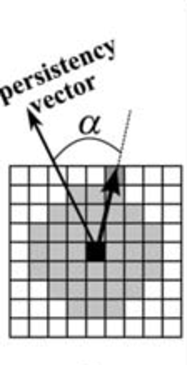
\includegraphics[width=0.15\textwidth]{persistency.pdf}\\
Here, $\alpha$ is the angle between the direction the cell wants to move in (the ``targetvector'') and the direction of the pixel copy being 
considered, as considered from the center of mass of the cell. $\mu$ modifies the strength of migration. First consider why the equation 
looks like this. Why the cosine? What happens for different directions of possible pixel copy events?\\

In addition to extending the Hamiltonian, cells in the model now have to keep track of their preferred direction of motion. Of course, they will 
often encounter obstacles, like other cells, and won't be able to move exactly in that direction. Rather than doggedly trying to keep moving there, 
cells will pause, change their course and continue in a different direction. The pause is thought to be caused by rearrangements of the actin cytoskeleton involved in migration. 
We implement this by changing the targetvector every 
\texttt{perstime} time steps to the actual direction in which the cell has been moving during that period.\\

For these exercises, use a bigger grid to give cells plenty of space to move. 400x400, with smaller cells (e.g. 30-50 for \texttt{targetvol}0 will do. Note that there is an initialisation period (300 steps) during which cells will not migrate yet!
\begin{itemize}
 \item Set \texttt{NrCellTypes} and \texttt{InitNrCells} to 1, and gradually increase \texttt{mu}($\mu$) and \texttt{perstime}. \\What do you notice about 
this lonely cell's pattern of movement?
\item Add more cells of the same cell type, and play with the initial configration and the adhesion between cells:\\
 either scattered randomly or clumped and either adhering to each other or not. \\What do you observe about 
their patterns of motion? How would this be relevant for e.g. collective cell migration in development, or T cell migration in lymph nodes?
\item Go back to some of the configurations you were trying to make in the previous section, but now add a bit of active migration (keep \texttt{mu} 
and \texttt{perstime} somewhat small). What do you observe, and why is that? How would this be relevant for development?
\end{itemize}
\nocite{*}
\vspace*{1cm}
Handy resources if you're interested in knowing more:
 \bibliography{refs.bib}
 \bibliographystyle{plain}


% \section{Extra: surface area constraint}
% Another extension is the surface area constraint, which set a target amount of membrane for each cell. This looks quite similar to the volume 
% constraint: 
% $$ H_{surf} = \sum_\sigma \lambda_s ( s_\sigma - S_{\tau(\sigma)}  )^2 $$
% Where $\lambda_s$ is the resistence of the cell to changes in its surface area (or, in the case of 2D cells, its perimeter), $s$ is the current 
% surface area and $S$ the target surface area. Be mindful of  the way in which the perimeter 
% is counted when you deal with this constraint. The length of the membrane  depends on the neighbourhood order you use
% 
% \item \textbf{extra: surfacearea constraint} Set \texttt{InitNrCells} back to 1, \texttt{surfaceconstraint} to 1 and \texttt{labdasurf} too. Change 
% \texttt{targetsurface}. What changes? Make sure to put \texttt{surfaceconstraint} back to 0 before proceeding.


\end{document}
